\documentclass{article}
\usepackage{tikz}
\usetikzlibrary{decorations.markings}
\pagestyle{empty}
\begin{document}
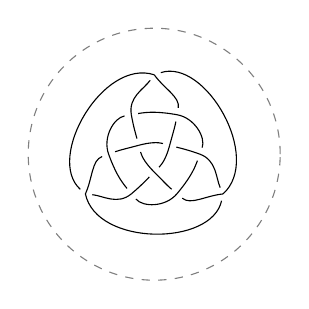
\begin{tikzpicture}
[scale=1.6,every node/.style={draw, circle, fill=white, inner sep=0pt, outer sep=0pt, minimum size=2.5pt},
->-/.style={decoration={markings, mark=at position .5 with{\arrow{>}}}, postaction={decorate}},
-<-/.style={decoration={markings, mark=at position .5 with{\arrow{<}}}, postaction={decorate}}]
\draw[gray, dashed] (0,0) circle (1.0);
 \node[draw=none, minimum size=0pt] (13) at (0.0,1.0) {};
\node[draw=none, minimum size=0pt] (14) at (-0.866025,-0.5) {};
\node[draw=none, minimum size=0pt] (15) at (0.866025,-0.5) {};
\node[minimum size=0pt] (1) at (-0.1815,0.3132) {};
\node[minimum size=0pt] (2) at (0.1815,0.3132) {};
\node[minimum size=0pt] (3) at (0.1227,0.0708) {};
\node[minimum size=0pt] (4) at (-0.0,0.6305) {};
\node[minimum size=0pt] (5) at (0.546,-0.3152) {};
\node[minimum size=0pt] (6) at (0.3619,6.0E-4) {};
\node[minimum size=0pt] (7) at (-0.546,-0.3152) {};
\node[minimum size=0pt] (8) at (-0.1805,-0.3137) {};
\node[minimum size=0pt] (9) at (0.1805,-0.3137) {};
\node[minimum size=0pt] (10) at (-0.3619,6.0E-4) {};
\node[minimum size=0pt] (11) at (-0.1227,0.0708) {};
\node[minimum size=0pt] (12) at (-0.0,-0.1416) {};
\draw[out=370.0, in=170.0, shorten <=2.5pt] (1) to (2);
\draw[out=460.0, in=594.0, shorten >=2.5pt] (1) to (4);
\draw[out=550.0, in=470.0, shorten <=2.5pt] (1) to (10);
\draw[out=280.0, in=465.0, shorten >=2.5pt] (1) to (11);
\draw[out=260.0, in=75.0, shorten <=2.5pt] (2) to (3);
\draw[out=350.0, in=430.0, shorten >=2.5pt] (2) to (6);
\draw[out=440.0, in=306.0, shorten <=2.5pt] (2) to (4);
\draw[out=165.0, in=375.0, shorten <=2.5pt] (3) to (11);
\draw[out=255.0, in=405.0, shorten >=2.5pt] (3) to (12);
\draw[out=345.0, in=520.0, shorten <=2.5pt] (3) to (6);
\draw[out=378.0, in=42.0, shorten <=2.5pt] (4) to (5);
\draw[out=522.0, in=498.0, shorten >=2.5pt] (4) to (7);
\draw[out=114.0, in=340.0, shorten <=2.5pt] (5) to (6);
\draw[out=186.0, in=320.0, shorten >=2.5pt] (5) to (9);
\draw[out=258.0, in=282.0, shorten <=2.5pt] (5) to (7);
\draw[out=610.0, in=410.0, shorten <=2.5pt] (6) to (9);
\draw[out=354.0, in=220.0, shorten <=2.5pt] (7) to (8);
\draw[out=426.0, in=560.0, shorten >=2.5pt] (7) to (10);
\draw[out=310.0, in=230.0, shorten <=2.5pt] (8) to (9);
\draw[out=400.0, in=225.0, shorten >=2.5pt] (8) to (12);
\draw[out=490.0, in=290.0, shorten <=2.5pt] (8) to (10);
\draw[out=500.0, in=315.0, shorten <=2.5pt] (9) to (12);
\draw[out=380.0, in=195.0, shorten <=2.5pt] (10) to (11);
\draw[out=285.0, in=135.0, shorten <=2.5pt] (11) to (12);
\end{tikzpicture}
\end{document}